% fs-03-Counting.tex

\documentclass[xcolor=dvipsnames]{beamer}

\usepackage{graphicx}
\usepackage{wrapfig}
\usepackage{colortbl}
\usepackage{alltt}
\definecolor{myblue}{rgb}{0.8,0.85,1}

\mode<presentation>
{
  \usetheme{Warsaw}
  \setbeamercovered{transparent}
}
% \usecolortheme[named=OliveGreen]{structure}
\setbeamertemplate{navigation symbols}{} 
\setbeamertemplate{blocks}[rounded][shadow=true] 

\newif\ifBCITCourse
\BCITCoursetrue
% \BCITCoursefalse
\newif\ifWhichCourse
\WhichCoursetrue
% \WhichCoursefalse
\ifBCITCourse
\ifWhichCourse
\newcommand{\CourseName}{Statistics for Food Technology}
\newcommand{\CourseNumber}{MATH 2441}
\newcommand{\CourseInst}{BCIT}
\else
\newcommand{\CourseName}{Calculus for Geomatics}
\newcommand{\CourseNumber}{MATH 2511}
\newcommand{\CourseInst}{BCIT}
\fi
\else
\newcommand{\CourseName}{Philosophy and Literature}
\newcommand{\CourseNumber}{PHIL 375}
\newcommand{\CourseInst}{UBC}
\fi

\title{Counting}
\subtitle{{\CourseNumber}, BCIT}

\author{\CourseName}

\date{January 23, 2017}

% \begin{figure}[h]
% 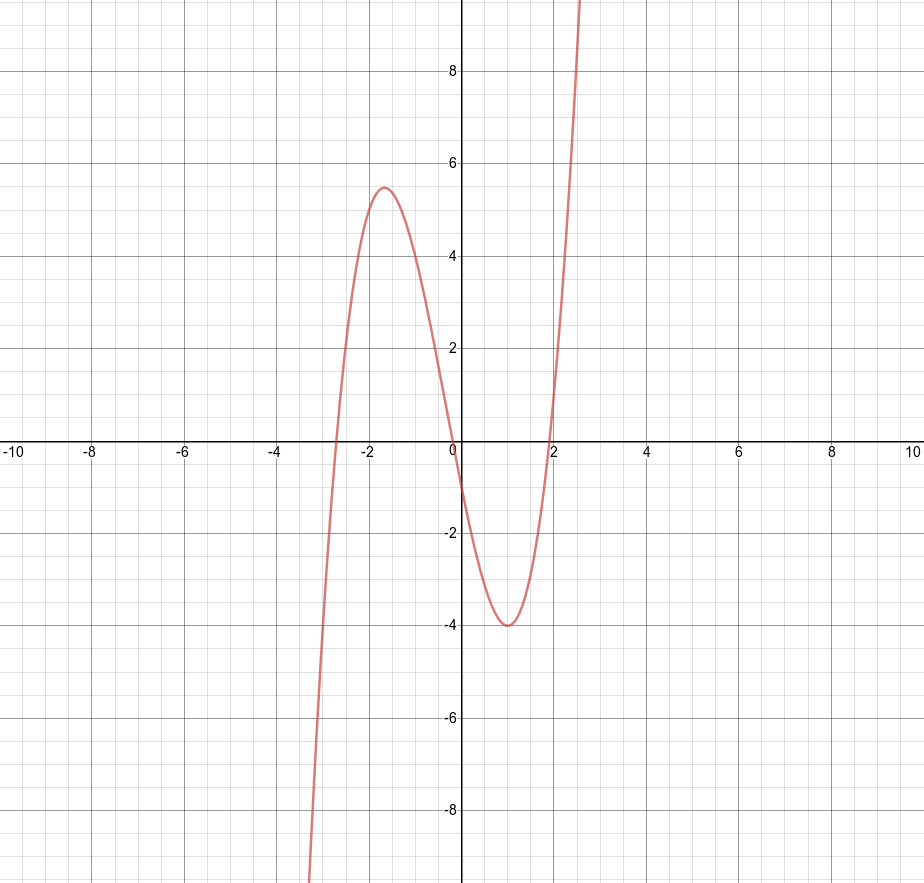
\includegraphics[scale=.3]{./diagrams/extrema1.png}
% \end{figure}

% Command             10pt    11pt    12pt
% \tiny               5       6       6
% \scriptsize         7       8       8
% \footnotesize       8       9       10
% \small              9       10      10.95
% \normalsize         10      10.95   12

\begin{document}

\begin{frame}
  \titlepage
\end{frame}

\begin{frame}
  \frametitle{How to Solve Probability Problems}
In summary, here are some strategies to solve probability problems.
\begin{enumerate}
\item Count simple events. If the simple events are all equally
  probable, then the probability of event $A$ is the number of simple
  events in $A$ divided by the total number of simple events, so
  $P(A)=\#A/\#\Omega$.
\item Make sure to watch for independence and mutual exclusion.
  Whenever events are independent or mutually exclusive (disjoint),
  you can use $P(A\cap{}B)=P(A)P(B)$ or $P(A\cup{}B)=P(A)+P(B)$,
  respectively.
\item If events are not mutually exclusive, you can use the
  addition rule $P(A\cup{}B)=P(A)+P(B)-P(A\cap{}B)$.
\item If events are not independent, you can use conditional
  probabilities in $P(A\cap{}B)=P(A)P(B|A)$.
\item If you are dealing with events that are independent and
  mutually exclusive, it is often useful to draw a tree diagram.
\end{enumerate}
\end{frame}

\begin{frame}
  \frametitle{Permutations and Combinations}
When we use
\begin{equation}
  \label{eq:adeiquah}
  P(A)=\frac{\#A}{\#\Omega}
\end{equation}
it can be difficult to do the counting. Formulas for permutations and
combinations help. For \alert{permutations}, order matters. The
permutations of the letters ABC are ABC, ACB, BAC, BCA, CAB, and CBA.
For \alert{combinations}, order does not matter. There are four
combinations of three letters for the four letters ABCD: ABC, ABD,
ACD, and BCD.
\end{frame}

\begin{frame}
  \frametitle{Rule I: Fundamental Counting Rule}
  The fundamental counting rule says that if there are $m$ ways for
  the first event to occur and $n$ ways for the second event to occur,
  then there are $m\cdot{}n$ combinations of these two events to
  occur.

\bigskip

\textbf{Example:} How many postal codes are possible in Canada?
\end{frame}

\begin{frame}
  \frametitle{Rule II: Factorial Rule}
Factorials are defined as follows,
\begin{equation}
  \label{eq:iepeejae}
  0!=1\mbox{ and }(n+1)!=(n+1)\cdot{}n!\mbox{ for all natural numbers }n
\end{equation}
For example, $6!=1\cdot{}2\cdot{}3\cdot{}4\cdot{}5\cdot{}6=720$.

\bigskip

The factorial rule says that there are $n!$ ways to arrange $n$
different items.

\bigskip

\textbf{Example:} You have to rank six Canadian prime ministers in
chronological order. If you know nothing about history, what is your
probability of ranking them correctly?
\end{frame}

\begin{frame}
  \frametitle{Rule III: Permutations Rule}
When you select $r$ items from $n$ available items \alert{without
  replacement}, then there are
\begin{equation}
  \label{eq:eahaikee}
  \frac{n!}{(n-r)!}
\end{equation}
permutations.

\bigskip

\textbf{Example:} How many ten-letter words are there without
repeating letters?
\end{frame}

\begin{frame}
  \frametitle{Rule IV: Combinations Rule}
When you select $r$ items from $n$ available items \alert{without
  replacement}, then there are
\begin{equation}
  \label{eq:aibireik}
  \frac{n!}{(n-r)!r!}
\end{equation}
combinations.

\bigskip

\textbf{Example:} How many different samples of $n=10$ are there in a
population of 30?
\end{frame}

\begin{frame}
  \frametitle{Counting Exercises I}
(1) When you steal someone's bank card and have to guess the 4-digit
PIN number (repetitions allowed), three attempts allowed, what is your
probability of success?
\end{frame}

\begin{frame}
  \frametitle{Counting Exercises II}
(2) How many four digit numbers are there with no repeating digits?
\end{frame}

\begin{frame}
  \frametitle{Counting Exercises III}
(3) If you were to read the seven Harry Potter books in random order,
what is the probability that you read them in the correct order?
\end{frame}

\begin{frame}
  \frametitle{Counting Exercises IV}
(4) The Rankin Family wants to make a Best Of CD out of their 27
songs. The CD is to have 12 songs on it. How many possibilities of
choosing 12 out of 27 songs are there (order does not matter)?
\end{frame}

\begin{frame}
  \frametitle{Counting Exercises V}
(5) Justin Trudeau wants to visit 4 out of the 10 Canadian provinces.
His advisor rattles off all the possible routes (order matters), one
per ten seconds. How long did it take her to do so?
\end{frame}

\begin{frame}
  \frametitle{Counting Exercises VI}
(6) Lotto 649 draws 6 out of 49 numbers (order does not matter). What
is your chance of winning? What is your chance of getting 5 numbers
correctly?
\end{frame}

\begin{frame}
  \frametitle{End of Lesson}
Next Lesson: Bayes and Conditional Probability.
\end{frame}

\end{document}
